% MATH 573 HW 4
% LUKE WUKMER

\documentclass[10pt]{article}

% note: some of these are extremely useful and i don't remember why :o
%\usepackage{savetrees} % disable custom geometry stuff if you do this
\usepackage{titling}    % contol over title & stuff
\usepackage{amsmath, amsthm, amssymb, amsfonts}
\usepackage{amsxtra, amscd, geometry, graphicx}
\usepackage{endnotes}
\usepackage{cancel}
\usepackage{wrapfig}    %inline figs
\usepackage{bm} %allows fancy stuff like bold greek in math mode
\usepackage{alltt}
\usepackage{enumerate} %more/easier control over lists, also see enumitem
%\usepackage[all,cmtip]{xypic}
\usepackage{mathrsfs}
\usepackage{listings}
\usepackage{caption}
%\usepackage{subfigure}
%\usepackage{subcaption}
%\usepackage[pdftex]{hyperref}
%\usepackage[dvips,bookmarks,bookmarksopen,backref,colorlinks,linkcolor={blue},citecolor={blue},urlcolor={blue}](hyperref}


\usepackage{color}

\definecolor{mygreen}{rgb}{0,0.6,0}
\definecolor{mygray}{rgb}{0.5,0.5,0.5}
\definecolor{mymauve}{rgb}{0.58,0,0.82}

\lstset{ %
  backgroundcolor=\color{white},   % choose the background color; you must add \usepackage{color} or \usepackage{xcolor}
  basicstyle=\footnotesize,        % the size of the fonts that are used for the code
  breakatwhitespace=false,         % sets if automatic breaks should only happen at whitespace
  breaklines=true,                 % sets automatic line breaking
  captionpos=b,                    % sets the caption-position to bottom
  commentstyle=\color{mygreen},    % comment style
  deletekeywords={...},            % if you want to delete keywords from the given language
  escapeinside={\%*}{*)},          % if you want to add LaTeX within your code
  extendedchars=true,              % lets you use non-ASCII characters; for 8-bits encodings only, does not work with UTF-8
  frame=single,	                   % adds a frame around the code
  keepspaces=true,                 % keeps spaces in text, useful for keeping indentation of code (possibly needs columns=flexible)
  keywordstyle=\color{blue},       % keyword style
  language=Python,                 % the language of the code
  otherkeywords={*,...},           % if you want to add more keywords to the set
  numbers=left,                    % where to put the line-numbers; possible values are (none, left, right)
  numbersep=5pt,                   % how far the line-numbers are from the code
  numberstyle=\tiny\color{mygray}, % the style that is used for the line-numbers
  rulecolor=\color{black},         % if not set, the frame-color may be changed on line-breaks within not-black text (e.g. comments (green here))
  showspaces=false,                % show spaces everywhere adding particular underscores; it overrides 'showstringspaces'
  showstringspaces=false,          % underline spaces within strings only
  showtabs=false,                  % show tabs within strings adding particular underscores
  stepnumber=2,                    % the step between two line-numbers. If it's 1, each line will be numbered
  stringstyle=\color{mymauve},     % string literal style
  tabsize=2,	                   % sets default tabsize to 2 spaces
  title=\lstname                   % show the filename of files included with \lstinputlisting; also try caption instead of title
}
% change up the fonts (pick one only)
%\usepackage{times}%
\usepackage{helvet}%
%\usepackage{palatino}%
%\usepackage{bookman}%


% These are italic.
\theoremstyle{plain}
\newtheorem{thm}{Theorem}
\newtheorem*{thm*}{Theorem}
\newtheorem{prop}{Proposition}
\newtheorem*{prop*}{Proposition}
\newtheorem{conj}{Conjecture}
\newtheorem*{conj*}{Conjecture}
\newtheorem{lem}{Lemma}
  \makeatletter
  \@addtoreset{lem}{thm}
  \makeatother 
\newtheorem*{lem*}{Lemma}
\newtheorem{cor}{Corollary}
  \makeatletter
  \@addtoreset{cor}{thm}
  \makeatother 
\newtheorem*{cor*}{Corollary}

%\newtheorem{lem}[thm]{Lemma}
%\newtheorem{remark}[thm]{Remark}
%\newtheorem{cor}[thm]{Corollary}
%\newtheorem{prop}[thm]{Proposition}
%\newtheorem{conj}[thm]{Conjecture}

% These are normal (i.e. not italic).
\theoremstyle{definition}
\newtheorem*{ack*}{Acknowledgements}
\newtheorem*{app*}{Application}
\newtheorem*{apps*}{Applications}
\newtheorem{defn}{Definition}
\newtheorem*{defn*}{Definition}
\newtheorem{eg}{Example}
  \makeatletter
  \@addtoreset{eg}{thm}
  \makeatother 
\newtheorem*{eg*}{Example}
\newtheorem*{egs*}{Examples}
\newtheorem{ex}{Exercise}
\newtheorem*{ex*}{Exercise}
\newtheorem*{quest*}{Question}
\newtheorem{rem}{Remark}
\newtheorem*{rem*}{Remark}
\newtheorem{rems}{Remarks}
\newtheorem*{rems*}{Remarks}
\newtheorem{prob}{Problem}
\newtheorem*{prob*}{Problem}
\newtheorem*{soln*}{Solution}
\newtheorem{soln}{Solution}


% New Commands: Common Math Symbols
\providecommand{\R}{\mathbb{R}}%
\providecommand{\N}{\mathbb{N}}%
\providecommand{\Z}{{\mathbb{Z}}}%
\providecommand{\sph}{\mathbb{S}}%
\providecommand{\Q}{\mathbb{Q}}%
\providecommand{\C}{{\mathbb{C}}}%
\providecommand{\F}{\mathbb{F}}%
\providecommand{\quat}{\mathbb{H}}%

% haha, i originally forked this template from one provided by my abstract
% algebra TA (back in 2012 or something). probably don't need most of these,
% huh. 

% New Commands: Operators
\providecommand{\Gal}{\operatorname{Gal}}%
\providecommand{\GL}{\operatorname{GL}}%
\providecommand{\card}{\operatorname{card}}%
\providecommand{\coker}{\operatorname{coker}}%
\providecommand{\id}{\operatorname{id}}%
\providecommand{\im}{\operatorname{im}}%
\providecommand{\diam}{{\rm diam}}%
\providecommand{\aut}{\operatorname{Aut}}%
\providecommand{\inn}{\operatorname{Inn}}%
\providecommand{\out}{{\rm Out}}%
\providecommand{\End}{{\rm End}}%
\providecommand{\rad}{{\rm Rad}}%
\providecommand{\rk}{{\rm rank}}%
\providecommand{\ord}{{\rm ord}}%
\providecommand{\tor}{{\rm Tor}}%
\providecommand{\comp}{{\text{ $\scriptstyle \circ$ }}}%
\providecommand{\cl}[1]{\overline{#1}}%
\providecommand{\tr}{{\sf trace}}%

\renewcommand{\tilde}[1]{\widetilde{#1}}%
\numberwithin{equation}{section}

% i like the squiggly ones more. add as needed

\renewcommand{\Psi}{\varPsi}

\newcommand*\rfrac[2]{{}^{#1}\!/_{#2}}

% a very fancy dot product \ip{f}{g}
\newcommand\ip[2]{ \left\langle {#1} , {#2} \right\rangle }

% "s.t." for math mode
\providecommand{\st}{\text{ s.t. }}

% \norm{f} and such, super useful
\newcommand{\norm}[1]{\left\lVert#1\right\rVert}

% determinant
%\newcommand{\det}[1]{\textsf{det}\left(#1\right)}

% jacobian
\providecommand{\J}{\textsf{J}}

% this makes the spacing between lines of font a little bigger
%\newcommand{\spacing}[1]{\renewcommand{\baselinestretch}{#1}\large\normalsize}
%\spacing{1.2}

\newcommand*\mcol[1]{\overset{\big\uparrow}{\underset{\big\downarrow}{#1}}}

% Makes the margin size a little smaller, i gots stuff to say
\geometry{letterpaper,margin=.8in}

% titling stuff (from package titling)
\posttitle{\par\end{center}}
\setlength{\droptitle}{-.5in}
% END PREAMBLE %%%%%%%%%%%%%%%%%%%%%%%%%
%%%%%%%%%%%%%%%%%%%%%%%%%%%%%%%%%%%%%%%%


\begin{document}

\title{Math 573 HW\textsuperscript{\#}4}
\author{Luke Wukmer}
\date{Fall 2015}
\maketitle \thispagestyle{empty} % remove the page number from the first page
\lstset{language=Python}

%%%% PROBLEM 1
\begin{prob}
    Let $f$ be the $2\pi$-periodic function determined by the formula
    \[
            f(x) = \left|{x}\right| \quad \text{for} \,   -\pi \leq x \leq \pi
    \]

\begin{enumerate}[(a)]
    \item Find the Fourier series of $f$.
    \item Show that the Fourier series converges absolutely to $f$.
\end{enumerate}
\end{prob}

\begin{soln*} %In the following discussion, we observe that $f(x)$ is an even function on ${[-\pi,\pi]}$.
    \begin{enumerate}[(a)]
        \item 
            We find the Fourier coefficients $c_n$ for the series
            $\hat{f}(\omega) = \sum_{-\infty}^\infty c_n e^{in\omega} $:
            \begin{align*}
                \text{for } n = 0, \quad
                c_0 &= \frac{1}{2\pi} \int_{-\pi}^{\pi} f(\omega) d\omega
                \,=\, \frac{1}{2\pi}\left[\,\frac{\pi}{2} + \frac{\pi}{2}\,\right]
                \,=\, \boxed{\frac{1}{2} = c_0} \\
                \text{and for } n \neq 0, \quad
                c_n &= \frac{1}{2\pi} \int_{-\pi}^{\pi} f(\omega) e^{- i n\omega} d\omega 
                    \,=\, \frac{1}{2\pi}
                        \left[ \int_{0}^{\pi} \omega e^{-in\omega} d\omega
                        + \int_{-\pi}^{0} \left(-\omega\right) e^{-in\omega} d\omega \right] \\
                        &= \frac{1}{2\pi}
                        \left[ \int_{0}^{\pi} \omega e^{-in\omega} d\omega
                        - \int_{-\pi}^{0} \omega e^{-in\omega} d\omega \right] \\
                \text{Via integration by parts, }   \int_a^b \omega e^{-in\omega} d\omega
                        &= \left.-\frac{1}{in} \omega e^{-in\omega}\right|_a^b 
                        - \left(-\frac{1}{in}\right)\int_a^b e^{-in\omega} d\omega \\
                        &= \frac{i}{n}\left[\, \omega e^{-in\omega}\Big|_a^b
                            + \frac{i}{n}e^{-in\omega}\Big|_a^b \, \right]
                            \,=\, \left.\frac{e^{-in\omega}(1+in\omega)}{n^2}\right|_a^b \\
                            \Longrightarrow \quad c_n \,=\, \cdots
                            &= \frac{1}{2\pi}\left[\, \int_0^\pi + \int_{-\pi}^{0} \,\right] \\
                            &= \frac{1}{2\pi n^2}
                                \left[ (-1)^n (1 + i\pi n) - 1 - 1 + (-1)^n (1 - i\pi n)\right] \\
                                &= \frac{1}{2\pi n^2} \left[ (-1)^n \cdot 2 - 2 \right]
                                = \boxed{\frac{{(-1)}^n - 1}{\pi n^2 } = c_n ,\, n\neq 0}
            \end{align*}
        Thus,
        \[
                \hat{f}(\omega) = \sum_{N=-\infty}^{\infty} c_n e^{in\omega}
                \; ,\;\text{where}\quad  c_n =
                \left\{\begin{array}{cr}
                        \rfrac{1}{2}                    & ,\, n = 0 \\[4pt]
                        \frac{{(-1)}^n - 1}{\pi n^2}    & ,\, n\neq 0
                    \end{array}\right.
            \]
                
        \item
            To show the Fourier series is absolutely convergent, we need to show
            $\displaystyle \sum_{N=-\infty}^\infty \left|\,{c_n} \right|$ is finite. 
            Using Bessel's inequality,
            \begin{align*}
                \sum_{-\infty}^{\infty}|c_n|^2
                    \leq \frac{1}{2\pi} \int_{-\pi}^{\pi} | f(\omega) |^2 d\omega
                    =\frac{1}{2\pi} \int_{-\pi}^{\pi} \omega^2 \,d\omega = \cdots = \frac{\pi^2}{3}
                    < \infty
                \end{align*}
            Then by the theorem, $S_f^N \rightarrow f$.
    \end{enumerate}
\end{soln*}

\hrulefill
\newpage
%%%% PROBLEM 2
\begin{prob}
    Prove that for any $N$,
    \[
            \int_{-\pi}^0  D_N(\omega) d\omega
        =   \int_{0}^{\pi}  D_N(\omega) d\omega = \frac{1}{2}
    \]
    where $D_N(\omega)$ is the $N^{\text{th}}$ Dirichlet kernel,
    $\displaystyle D_N(\omega) = \frac{1}{2\pi}\sum_{-N}^N e^{inw}$\,\,.
\end{prob}
\begin{soln*}
    %If  $N = 0$, we have $\displaystyle D_0(\omega) = \frac{1}{2\pi}$.
    Suppose $N\neq 0$. Then, by reorganizing,
    \begin{align*}
        \int_0^\pi D_N(\omega)d\omega &=
        \frac{1}{2\pi} \int_0^\pi \sum_{n=1}^{|N|}\left[
        e^{in\omega} + e^{-in\omega}\right] d\omega + \frac{1}{2\pi}\int_0^\pi e^{i(0)\omega} d\omega \\
        &= \frac{1}{2\pi} \sum_{n=1}^{|N|}\int_0^\pi \left[
        e^{in\omega} + e^{-in\omega}\right] d\omega + \frac{1}{2\pi}\int_0^\pi d\omega \\
        &= \frac{1}{2\pi} \sum_{n=1}^{|N|}
            \left[ \frac{1}{in} e^{in\omega} -\frac{1}{in} e^{-in\omega}\right]_0^\pi
            + \frac{1}{2} \\ 
        &= \frac{1}{2\pi} \sum_{n=1}^{|N|}
            \left[ \frac{1}{in}\left(
            \left(e^{i\pi}\right)^n - \left(e^{i\pi}\right)^{-n} - 1 + 1
        \right)\right] + \frac{1}{2}\\
        &= \frac{1}{2\pi} \sum_{n=1}^{|N|}
        \left[ \frac{1}{in}\left( (-1)^n - (-1)^{-n}\right)\right] + \frac{1}{2} 
        \,=\, 0 + \frac{1}{2} \,=\, \frac{1}{2}
    \end{align*}
    From the above it is clear that if $N=0$, the first term is nonexistent, and thus
    $\int_0^\pi D_0(\omega) d\omega = \frac{1}{2}$ as well.

    Finally, to show $\int_{-\pi}^0  D_N(\omega) d\omega =   \int_{0}^{\pi}  D_N(\omega) d\omega$,
    note that $\int_{-\pi}^{0} D_N(\omega) d\omega = \int_0^\pi D_N(-\omega) d\omega$.
    The first term is simply reordered and still cancels out, whereas the second term is unaffected,
    and we have the result.
    \qed
\end{soln*}

\hrulefill
%%%% PROBLEM 3

\begin{prob}
Show that for any functions $f,g,h$ on $\R$, $f\star (g \star h) = (f\star g) \star h$, where
\[
        f \star g(x) = \int f(x-y) g(y) dy
    \]
\end{prob}

\begin{soln*}
    From lecture, we know convolution is commutative, i.e. $f\star g = g \star f$.
    We apply this result several times in the following:
    \begin{align*}
        (f \star g ) \star h
        &= \int \left(f \star g(x-y)\right) h(y) dy = \int \left(g \star f(x-y)\right) h(y) dy \\
        &= \int \left[ \int g(x-y-\tau) f(\tau) d\tau \right] h(y) dy \\ \tag{\textbf{\maltese}}
        &= \int \int g(x-y-\tau) f(\tau) h(y) d\tau dy \\ 
        &= \int \left[ \int g(x-\tau-y) h(y) dy \right]f(\tau) d\tau  \\
        &= \int g\star h(x-\tau) f(\tau) d\tau = (g \star h) \star f = f \star (g \star h)
    \end{align*}
    Since both convolution integrals exist, we may apply Fubini's theorem in
    (\textbf{\maltese}) to freely change the order of integration.
    \qed
\end{soln*}

\hrulefill
\newpage
%%%%PROBLEM 4
\begin{prob}[Linear filtering for image denoising]
    A program for denoising the image \texttt{lena\_noisy.png} was developed in \texttt{p4.py}
    For this task, we employ a gaussian function
    \[
        g_\sigma(x,y) = 1 - e^{-\frac{(x-a)^2 + (y-b)^2}{2\sigma^2}}
    \]
    where $\sigma $ is the variance of the gaussian function and $(a,b)$ is the center of the peak.
    This is discretized over the size of the original image, with the center as the midpoint of the
    image, as implemented in the function \texttt{gaussian\_filter(...)}.
    \lstinputlisting[firstline=67, lastline=114]{p4.py}
    A 3D plot of this function is shown in \textbf{Figure 2} with variance $\sigma=15$.
    
    \newpage

    After we convert the original image into a 2D array, we use this filter by applying it
    to the fourier transform of the original image:
    \lstinputlisting[firstline=139, lastline=152]{p4.py}
    
    The results of this procedure are shown in \textbf{Figure 1}. Our choice for this particular
    was entirely heuristic. Higher variances allow for more sharply defined edges (i.e. features) to
    remain in the filtered image, at the cost of increased noise. Meanwhile,
    lower variances reduce noise more significantly, at the cost of blurred edges / reduced features.
    The empirical determination of an appropriate value for $\sigma$ is explored in
    \textbf{Figure 3--4}. The relevant code can be found in the file \texttt{p4\_varspread.py}.

    \begin{figure}[p]
    \begin{center}
        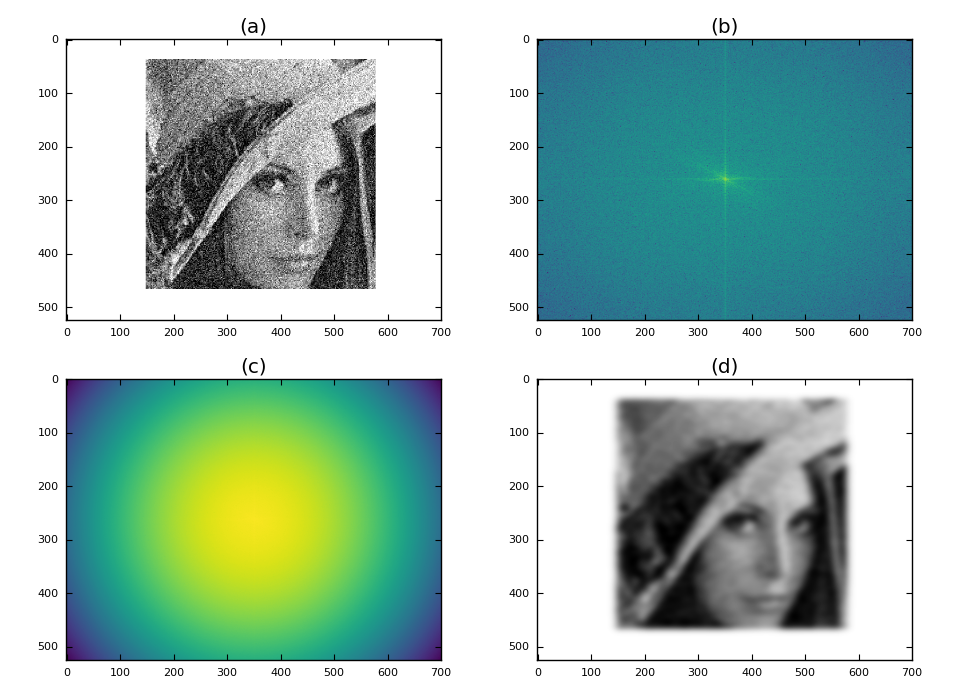
\includegraphics[width=0.8\textwidth]{prob4}
        \caption{
            \textbf{(a)} The original image.
            \textbf{(b)} A logarithmic colormap of the (absolute value) of the fourier spectrum of the image.
            \textbf{(c)} A discrete gaussian kernel with $\sigma=15$ is applied to the spectrum obtained in (b).
            \textbf{(d)} The resulting filtered image, which is the inverse fourier transform of the spectrum
                         represented in (c).
                     }
    \end{center}
\end{figure}
\begin{figure}[p]
    \begin{center}
        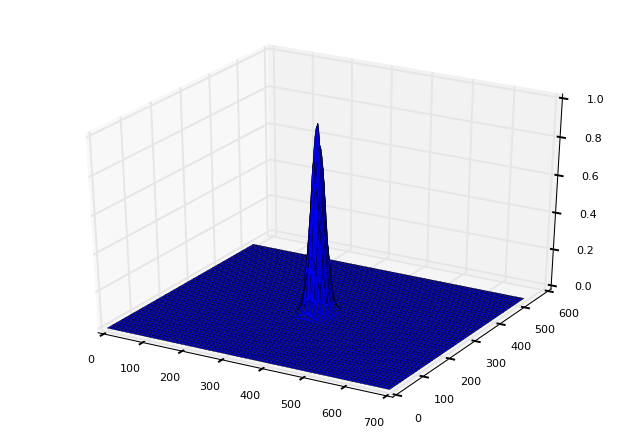
\includegraphics[width=0.8\textwidth]{p4-gaussian15}
        \caption{A 3D representation of the Gaussian function (with $\sigma=15$) used to filter.}
    \end{center}
\end{figure}
\begin{figure}[p]
    \begin{center}
        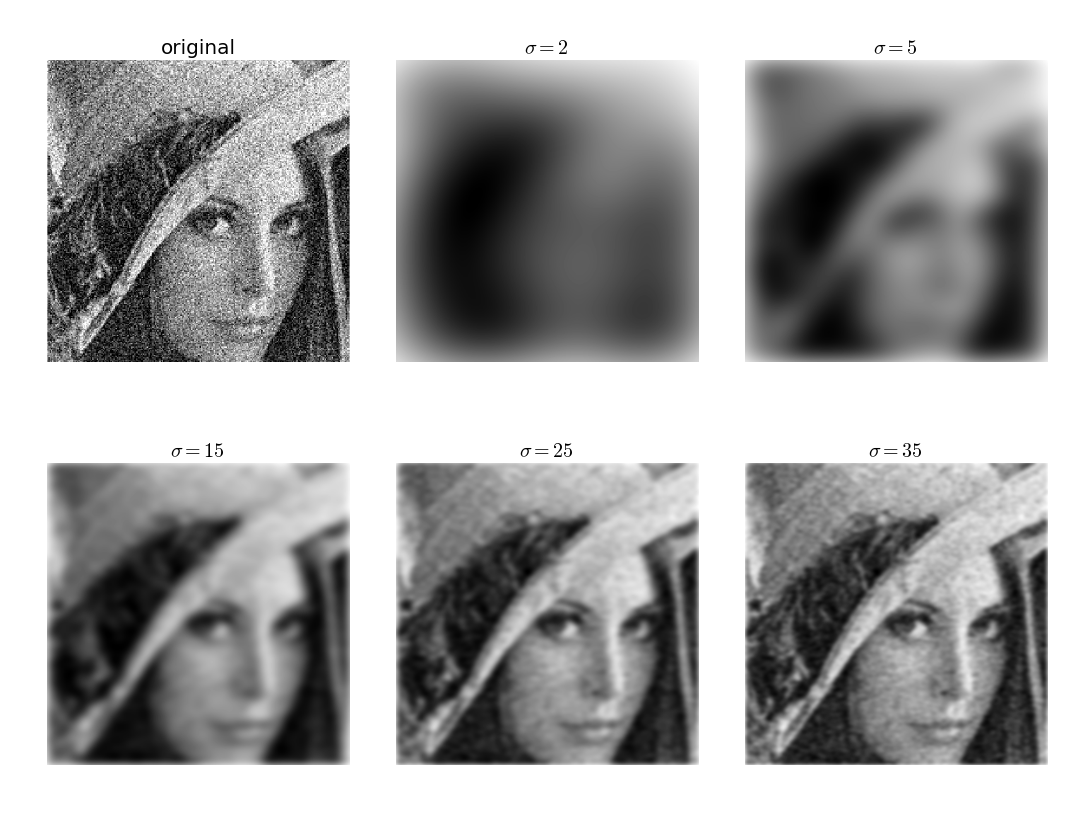
\includegraphics[width=0.8\textwidth]{varspread}
        \caption{
            A gaussian filter with variance $\sigma$ is applied to the source image \textbf{(original)}.
            The remaining images are result of gaussian filtering with variance
            $\sigma=2,5,15,25,35$. With low variance (e.g. $\sigma=2,5$),
            almost all detail (i.e. edges) is lost, but none of the original noise is present.
            Higher variances (e.g. $\sigma=25,35$) allow retention of edges, but also retain some of the
            original noise. A suitable value for $\sigma$ will compromise between these two extremes:
            in this case, choosing $\sigma=15$ allows for a significant reduction of the original noise
            while still retaining the defining features/edges of the original.
        }
    \end{center}
\end{figure}

\begin{figure}[p]
    \begin{center}
        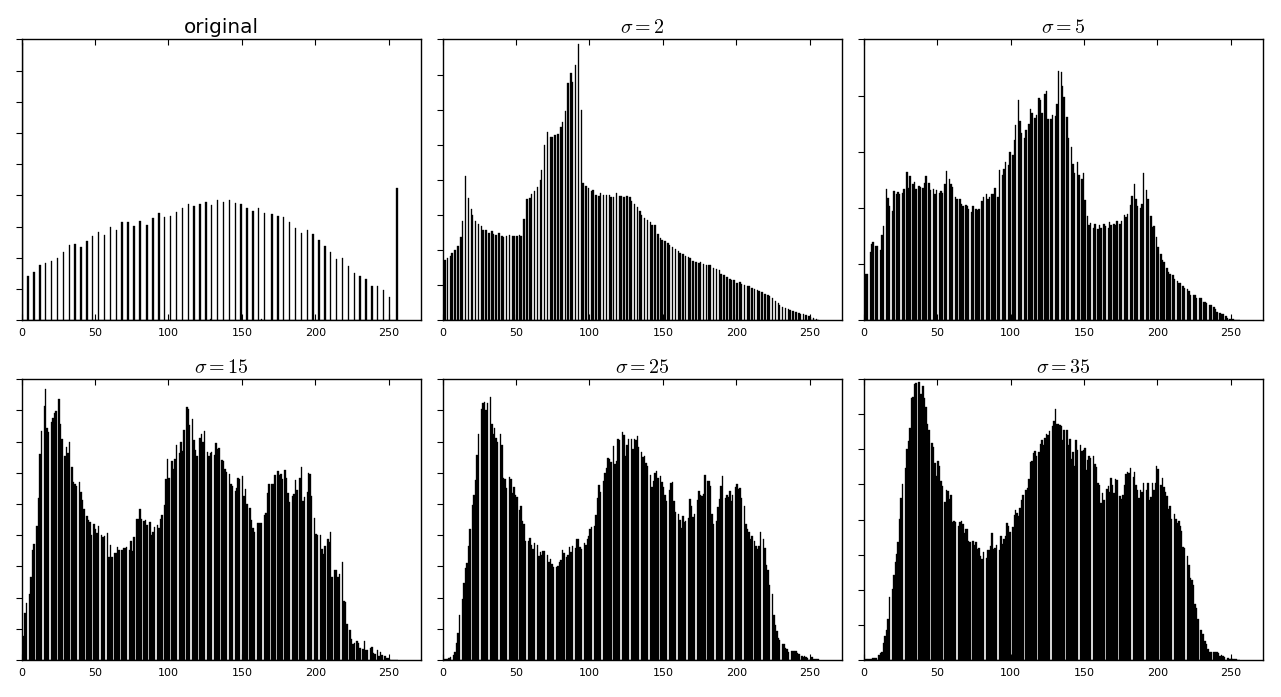
\includegraphics[width=0.8\textwidth]{varspread-hists}
        \caption{
            Histograms of each image in \textit{Figure 3}. We see that in all cases, the most
            extreme frequencies are removed (notice the prominent spike at 255 (white) in the histogram
            of the original image and its absense in the remaining histograms). Higher variances
            (e.g. $\sigma=15,25,35$) emphasize more of the lowest frequency content
            and highest frequency content--this translates to better defined edges, but more of the
            original noise retained. Lower variances (e.g. $\sigma=2,5$) result in a clear spike in a
            particular range, at the expense of either extreme. Note that
            these histograms only contain
            pixel values of the central the image itself without a border; that is, the original white border present
            (see \textit{Figure 1(a,d)}) has been removed.
        }
    \end{center}
\end{figure}

\end{prob}

\hrulefill
\clearpage
%%%%PROBLEM 5
\begin{prob}[Hybrid images]
    In \texttt{hybrid.py}, we use the techniques developed in four to create \textit{hybrid images}.
    These are images which incorporate the high frequency content of one image
    with the low frequency content of another. In short, the gaussian filter used in 
    \textbf{Problem 4} acts as a low-pass filter on the first image. A simple high-pass filter was created by
    simply reversing the gaussian function on its range ${[0,1]}$:
    \[
            \tilde{g}_\sigma(x,y) = 1 - g_\sigma(x,y) = 1 - e^{-\frac{(x-a)^2 + (y-b)^2}{2\sigma^2}}
        \]
    By combining these two images, a resulting image is created that visually appears
    similar to the low-passed image when viewed up close, and visually appears similar to the
    low-passed image when viewed from far away. This phenomenon is demonstrated first in
    \textbf{Figure 5}, where a hybrid image is created from well-known portraits of Albert
    Einstein and Marilyn Monroe. The gaussian functions used both have variance $\sigma=10$, which 
    was found empirically to best demonstrate this phenomenon.
    The implementation of this is very similar to that of the previous problem,
    performing the filtering procedure on both images simulatneously and adding the results:
    \lstinputlisting[firstline=26, lastline=53]{hybrid.py}
    \textbf{Figure 6} demonstrates the
    same phenomenon on a different set of images,
    the iconic "Blue Marble" taken from Apollo 17 in 1972, and a cat. The gaussian function used here
    has variance $\sigma=15$, again found empirically. The corresponding code (almost identical)
    can be found in \texttt{hybrid\_alt.py}.
    \begin{figure}[p]
    \begin{center}
        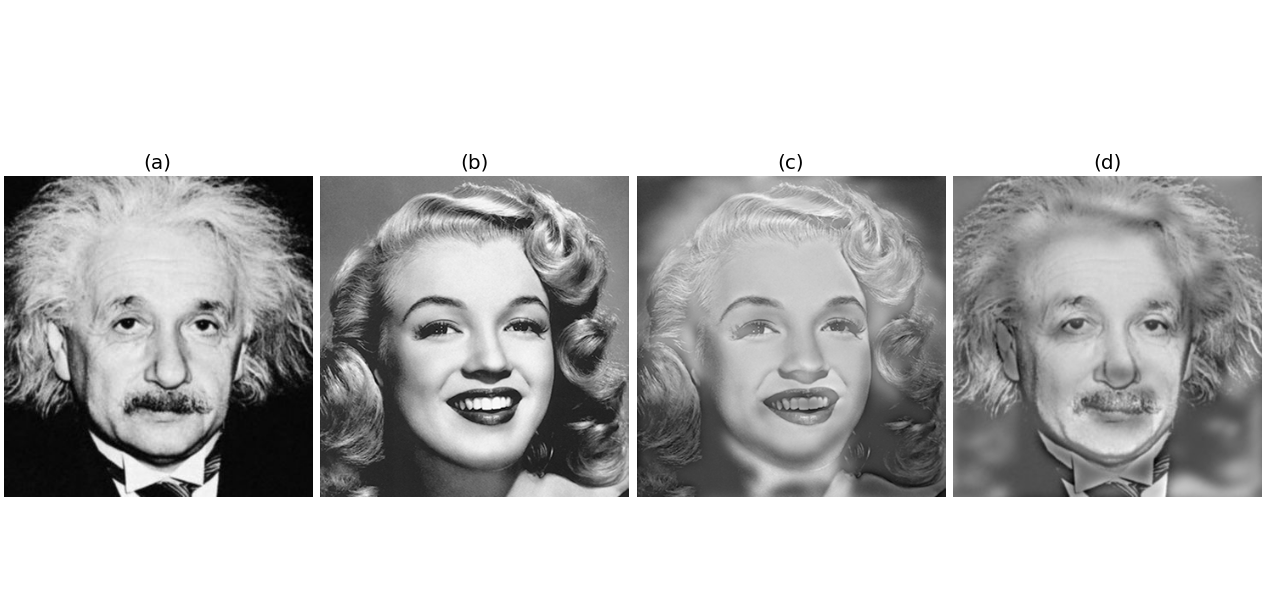
\includegraphics[width=\textwidth]{prob5}
        \caption{
        A demonstration of \textit{hybrid images}: The original images of Albert Einstein \textbf{(a)} and
        Marilyn Monroe \textbf{(b)} are hybridized: In \textbf{(c)}, the high pass filter has been
        applied to Marilyn, while a low pass filter has been applied to Albert.
        In \textbf{(d)}, these filters are reversed. In all cases, the gaussian function in question
        has variance $\sigma=10$, which was chosen empirically to best demonstrate this result.
            }
    \end{center}
\end{figure}

\begin{figure}[p]
    \begin{center}
        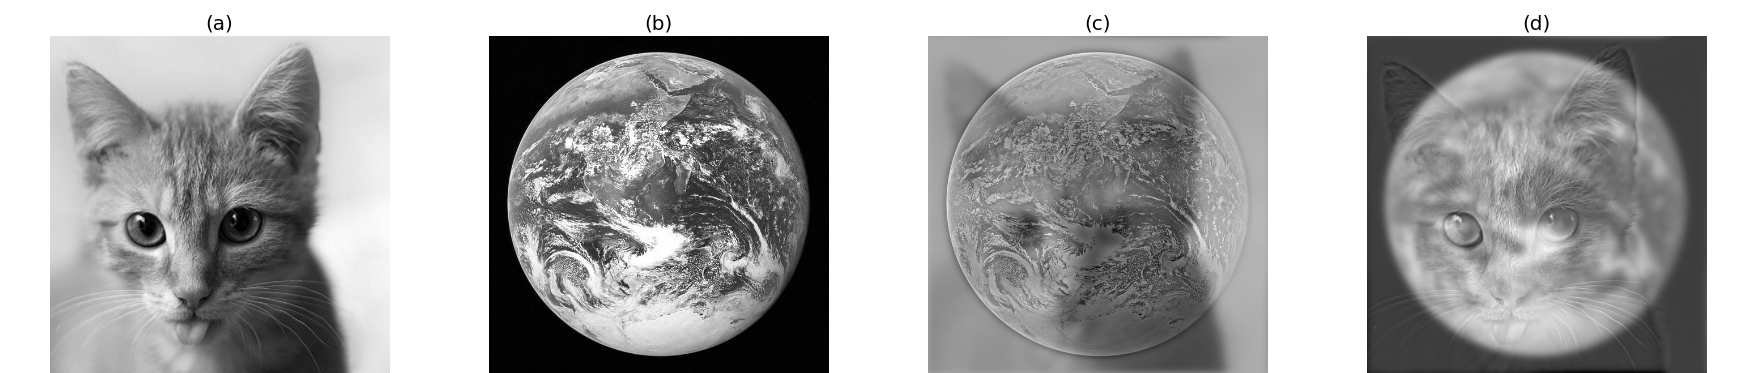
\includegraphics[width=\textwidth]{earthblep}
        \caption{
        Hybrid images were created in the same fashion as in \textit{Figure 5}
        with two different initial images, a blep \textbf{(a)}, and the iconic picture
        of planet earth \textbf{(b)}. \textbf{(c)} contains the high passed content on earth
        (which can be seen from the clear outlines of the planet and its cloud layer),
        while \textbf{(d)} contains the high-passed content of the cat (the clear outline of its eyes).
        In this case, the gaussian function was chosen to have variance $\sigma=15$.
    }
    \end{center}
\end{figure}
\end{prob}
\end{document}
